\documentclass{article}
\usepackage{amsmath}
\usepackage{amssymb}
\usepackage{amsfonts}
\usepackage{paracol}
\usepackage[inline]{enumitem}
\usepackage{geometry}
\usepackage{tikz}
\usetikzlibrary{angles,quotes}
\usetikzlibrary{datavisualization.formats.functions}
\renewcommand{\arraystretch}{1.2}
\geometry{a4paper, left=15mm, top=15mm, right=15mm, bottom=15mm}
\title{Chapter 18

  Advanced Trigonometry}
\date{}
\begin{document}
\maketitle
\section{Radian and Degree Measures}
\subsection{Convert them into degree measure}
\paragraph{Example 1:}
\begin{enumerate}
        \begin{paracol}{3}
          \item[a.] $\frac{\pi}{6}$
          \item[d.] $\frac{7\pi}{6}$
          \item[g.] $\frac{7\pi}{18}$
          \switchcolumn
          \item[b.] $\frac{4\pi}{5}$
          \item[e.] $\frac{8\pi}{3}$
          \switchcolumn
          \item[c.] $\frac{11\pi}{6}$
          \item[f.] $\frac{7\pi}{4}$
          \switchcolumn
        \end{paracol}
\end{enumerate}
{\footnotesize Since $\pi=180^{\circ}$, $1 radian = \frac{180^{\circ}}{\pi}$ OR $1^{\circ} = \frac{\pi}{180^{\circ}}$}

\paragraph{Solutions:}
\begin{enumerate}
        \begin{paracol}{3}
          \item[a.] $\frac{\pi}{6} \times \frac{180^{\circ}}{\pi} = 30^{\circ}$
          \item[d.] $\frac{7\pi}{6} \times \frac{180^{\circ}}{\pi} = 210^{\circ}$
          \item[g.] $\frac{7\pi}{18} \times \frac{180^{\circ}}{\pi} = 70^{\circ}$
          \switchcolumn
          \item[b.] $\frac{4\pi}{5} \times \frac{180^{\circ}}{\pi} = 144^{\circ}$
          \item[e.] $\frac{8\pi}{3} \times \frac{180^{\circ}}{\pi} = 480^{\circ}$
          \switchcolumn
          \item[c.] $\frac{11\pi}{6} \times \frac{180^{\circ}}{\pi} = 330^{\circ}$
          \item[f.] $\frac{7\pi}{4} \times \frac{180^{\circ}}{\pi} = 315^{\circ}$
          \switchcolumn
        \end{paracol}
\end{enumerate}

\subsection{Convert them to radian measure}
\paragraph{Example 2:}
\begin{enumerate}
        \begin{paracol}{3}
          \item[a.] $\theta=5^{'}$
          \item[d.] $330^{\circ}$
          \item[g.] $520^{\circ}$
          \switchcolumn
          \item[b.] $-120^{\circ}$
          \item[e.] $480^{\circ}$
          \item[h.] $240^{\circ}$
          \switchcolumn
          \item[c.] $210^{\circ}$
          \item[f.] $-47^{\circ}30^{'}$
          \item[i.] $-7^{\circ}30^{'}$
          \switchcolumn
        \end{paracol}
\end{enumerate}

\paragraph{Solutions :}
\begin{enumerate}
        \begin{paracol}{3}
          \item[a.] $\theta=5^{'}=\frac{5^{\circ}}{60} \times \frac{\pi}{180^{\circ}} = \frac{\pi}{12 \times 180} radians$
          \item[d.] $330^{\circ} = 330^{\circ} \times \frac{\pi}{180^{\circ}} = \left(\frac{11\pi}{6}\right)^{c}$
          \item[g.] $520^{\circ} = -520 \times \frac{\pi}{180^{\circ}} = \frac{26\pi}{9} $
          \switchcolumn
          \item[b.] $-120^{\circ} \times \frac{\pi}{180^{\circ}} = \left(\frac{-2 \pi}{3}\right)^{c}$
          \item[e.] $480^{\circ} = 480^{\circ} \times \frac{\pi}{180^{\circ}} = \frac{8\pi}{3}$
          \item[h.] $240^{\circ} = 240^{\circ} \times \frac{\pi}{180^{\circ}} = \frac{4\pi}{3}$
          \switchcolumn
          \item[c.] $210^{\circ} = 210^{\circ} \times \frac{\pi}{180^{\circ}} = \frac{7\pi}{6}$
          \item[f.] $-47^{\circ}30^{'} = -47\frac{1}{2}^{\circ} \\
          = \left(\frac{-95}{2}^{\circ}\right) \times \frac{\pi}{180^{\circ}} \\
          = \frac{-19\pi}{72} $
          \item[i.] $-7^{\circ}30^{'} = 7\frac{1}{2}^{\circ} \\
          = 7\frac{1}{2}^{\circ} \times \left(\frac{\pi}{180}\right)^{c} \\
          = \frac{15}{2} \times \left(\frac{\pi}{180}\right)^{c} \\
          = \left(\frac{\pi}{24}\right)^{c}$
          \switchcolumn
        \end{paracol}
\end{enumerate}

\subsection{Sine, Cosine and Tangents}
\paragraph{Example 3: Without using calculator, solve the following questions}
\begin{enumerate}[label=\alph*)]
  \item If $\sin(18^{\circ})= 0.309$, give another angle whose $\sin$ is $0.309$.
        
        {\scriptsize \textbf{Solution:} since}
        \[
        \begin{aligned}
          \sin(180^{\circ}-\theta) = \sin(\theta)
          &\therefore \sin(180^{\circ}-18^{\circ}) = \sin(162^{\circ}) \\
          &\therefore \theta = 162^{\circ}
        \end{aligned}
        \]

  \item If $\cos(70^{\circ})= 0.342$, give another angle whose $\cos$ is $0.342$.

        {\scriptsize \textbf{Solution:} since}
        \[
        \begin{aligned}
          \cos\theta = \cos(2\pi - \theta)
          &\therefore \cos(360-70^{\circ}) = \cos(290^{\circ}) \\
          &\therefore \theta = 290^{\circ}
        \end{aligned}
        \]

  \item If $\cos(300^{\circ})= \frac{1}{2}$, give another angle whose $\cos$ is $\frac{1}{2}$.

        {\scriptsize \textbf{Solution:} since}
        \[
        \begin{aligned}
          \cos(300^{\circ}) &= \cos(360-60^{\circ}) = \cos(60^{\circ}) \\
                       &\therefore \theta = 60^{\circ}
        \end{aligned}
        \]

  \item If $\cos(120^{\circ})= \frac{-1}{2}$, give another angle whose $\cos$ is $-0.5$.

        {\scriptsize \textbf{Solution:} since}
        \[
        \begin{aligned}
          \cos\theta = \cos(360-\theta)
          &\therefore \cos(120^{\circ}) = \cos(360^{\circ} - 120^{\circ}) = \cos(240^{\circ}) \\
          &\therefore \theta = 240^{\circ}
        \end{aligned}
        \]

  \item (Use Calculator) If $\sin(x)= 0.848$, find two values for $x$ between $0^{\circ}$ and $360^{\circ}$.

        \[
        \begin{aligned}
          x = 58^{\circ}, 122^{\circ}
        \end{aligned}
        \]
\end{enumerate}

\paragraph{Example 4:}
If $\tan\theta = \frac{1}{\sqrt{3}}$, find the other values of a) $\sin\theta$ b) $\cos\theta$

{\scriptsize \textbf{Solutions:}}
\begin{enumerate}[label=\alph*)]
        \item
        \[
        \begin{aligned}
          \sec^{2}\theta = \tan^{2}\theta + 1 = \frac{1}{3}+1 = \frac{4}{3} \\
          \therefore \sec\theta = \pm\frac{2}{\sqrt{3}} \Rightarrow \cos\theta = \pm \frac{\sqrt{3}}{2}
        \end{aligned}
        \]

        \item
        \[
        \begin{aligned}
          \sin\theta^{2}\theta = 1 - \cos^{2}\theta = 1 - \frac{3}{4} = \frac{1}{4} \\
          \therefore \sin\theta = \pm\frac{1}{2}
        \end{aligned}
        \]
\end{enumerate}

\paragraph{Example 5:}
If $\sin\theta = \frac{1}{\sqrt{2}}$, find the values of a) $\cos\theta$ b) $\tan\theta$

{\scriptsize \textbf{Solutions:}}
\begin{enumerate}[label=\alph*)]
        \item
        \[
        \begin{aligned}
          \cos^{2}\theta = 1 - \sin^{2}\theta = 1 - \frac{1}{2} = \frac{1}{2} \\
          \cos\theta = \pm\frac{1}{\sqrt{2}} \\
        \end{aligned}
        \]

        \item
        \[
        \begin{aligned}
          \tan\theta = \frac{\sin\theta}{\cos\theta} = \frac{1/\sqrt{2}}{\pm\frac{1}{\sqrt{2}}} = \pm 1
        \end{aligned}
        \]
\end{enumerate}

Alternatively, we can find these values by drawing a right angle triangle.

\begin{center}
  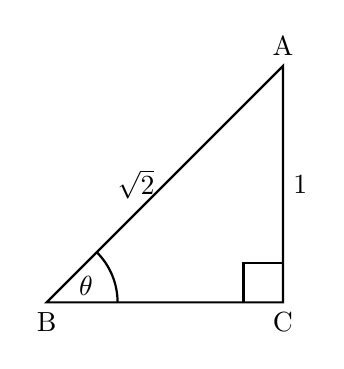
\begin{tikzpicture}[thick]
    % Draw the triangle
    \coordinate (A) at (3,3);
    \coordinate (B) at (0,0);
    \coordinate (C) at (3,0);

    \draw (A) -- node[midway, left]{$\sqrt{2}$}
    (B) --
    (C) -- node[midway, right]{$1$} cycle;

    % more labels
    \node[above] at (A) {A};
    \node[below] at (B) {B};
    \node[below] at (C) {C};

    % draw angles
    \pic [draw, angle radius=9mm, "$\theta$"] {angle = C--B--A};
    \pic [draw] {right angle = A--C--B};
  \end{tikzpicture}
\end{center}

{\scriptsize \textbf{Solution:}}
\[ \sin\theta = \frac{1}{\sqrt{2}} \]
Applying Pythagoras theorem
\[
  \begin{aligned}
    BC^{2} = AB^{2} - AC^{2} = 2 - 1 = 1 \\
    BC = 1
  \end{aligned}
\]
$\therefore$

\[
  \begin{aligned}
    \cos\theta = \frac{BC}{AB} = \frac{1}{\sqrt{2}} \\
    \tan\theta = \frac{AC}{BC} = \frac{1}{1} = 1
  \end{aligned}
\]

\subsection{Verifying Trigonometric Identities}
\paragraph{Example 6: Verify each of the following by putting values}

\begin{enumerate}[label=\alph*)]
  \item $\sin 60^{\circ} \cos 30^{\circ} - \cos 60^{\circ} \sin 30^{\circ} = \sin 30^{\circ} \Rightarrow \frac{\sqrt{3}}{2} \times \frac{\sqrt{3}}{2} - \frac{1}{2} \times \frac{1}{2} = \frac{3-1}{4}=\frac{1}{2}$
  \item $\cos 60^{\circ} \cos 30^{\circ} + \sin 60^{\circ} \sin 30^{\circ} = \cos 30^{\circ} \Rightarrow \frac{1}{2} \times \frac{\sqrt{3}}{2} + \frac{\sqrt{3}}{2} \times \frac{1}{2} = \frac{\sqrt{3}}{2}$
  \item $2 \sin 30^{\circ} \cos 30^{\circ} = \sin 60^{\circ} \Rightarrow 2 \times \frac{1}{2} \times \frac{\sqrt{3}}{2} = \frac{\sqrt{3}}{2}$
  \item $\cos 60^{\circ} = 2 \cos^{2} 30^{\circ} - 1 \Rightarrow 2 \times \left(\frac{\sqrt{3}}{2}\right)^{2} - 1 = 2 \times \frac{3}{4} - 1 = \frac{1}{2}$
  \item $\cos 60^{\circ} = 1 - 2 \sin^{2} 30^{\circ} \Rightarrow 1 - 2 \times \left(\frac{1}{2}\right)^{2} = 1 - \frac{1}{2} = \frac{1}{2}$
\end{enumerate}

\paragraph{Example 7:}
Using the formula $\cos A = \sqrt\frac{1+\cos2A}{2}$ and $\sin A = \sqrt\frac{1-\cos2A}{2}$
find the value of $\cos30^{\circ}$ and $\sin30^{\circ}$.

{\scriptsize \textbf{Solution:}}

\[
  \begin{aligned}
    \cos30^{\circ} = \sqrt\frac{1+\cos60^{\circ}}{2} =  \sqrt\frac{1+\frac{1}{2}}{2} = \sqrt\frac{3}{4} = \frac{\sqrt{3}}{2} \\
    \sin30^{\circ} = \sqrt\frac{1-\cos60^{\circ}}{2} =  \sqrt\frac{1-\frac{1}{2}}{2} = \sqrt\frac{1}{4} = \frac{1}{2} \\
  \end{aligned}
\]

\paragraph{Example 8:}
If $A = 60^{\circ}, B = 30^{\circ}$, verify

\begin{enumerate}[label=\alph*)]
  \item $\sin(A-B) = \sin(A) \cos(B) - \cos(A) \sin(B)$
  \item $\cos(A-B) = \cos(A) \cos(B) - \sin(A) \sin(B)$
  \item $\tan(2A) = \frac{2\tan(A)}{1-\tan^{2}(A)}$
\end{enumerate}

{\scriptsize \textbf{Solutions:}}

\begin{enumerate}[label=\alph*)]
  \item $\sin(60^{\circ}-30^{\circ}) = \sin60^{\circ}\cos30^{\circ} - \cos60^{\circ}\sin30^{\circ}$ \\
        $ \frac{1}{2} = \frac{\sqrt{3}}{2} \times \frac{\sqrt{3}}{2} - \frac{1}{2} \times \frac{1}{2} = \frac{3}{4} - \frac{1}{4} = \frac{1}{2} $
  \item $\cos(60^{\circ}-30^{\circ}) = \cos60^{\circ}\cos30^{\circ} + \sin60^{\circ}\sin30^{\circ}$ \\
        $ \frac{\sqrt{3}}{2} = \frac{1}{2} \times \frac{\sqrt{3}}{2} + \frac{\sqrt{3}}{2} \times \frac{1}{2} = 2 \times \frac{\sqrt{3}}{4} = \frac{\sqrt{3}}{2}$
  \item $\tan(2A) = \frac{2\tan(A)}{1-\tan^{2}(A)}$ \\
        $ \tan 60^{\circ} = \frac{2\tan30^{\circ}}{1-\tan^{2}30^{\circ}} = \frac{2\frac{1}{\sqrt{3}}}{1-\frac{1}{3}} = \frac{2\frac{1}{\sqrt{3}}}{\frac{2}{3}} = \sqrt{3} \frac{\sqrt{3}}{\sqrt{3}} = \sqrt{3}$ \\
        $\therefore \sqrt{3} = \sqrt{3}$
\end{enumerate}

\paragraph{Example 9:}
If $A = 30^{\circ}$, verify $\cos3A = 4\cos^{3}A - 3 \cos(A) $ and $\sin3A = 3\sin(A) - 4\sin^{3}A$

{\scriptsize \textbf{Solution:}}

\[
  \begin{aligned}
    \cos(3 \times 30^{\circ}) &= 4\cos^{3}30^{\circ} - 3\cos30^{\circ} \\
                         &= 4\left(\frac{\sqrt{3}}{2}\right)^{2} - 3\frac{\sqrt{3}}{2} \\
                         & 0 = 4 \times \frac{3\sqrt{3}}{4\times2} - \frac{3\sqrt{3}}{2} = 0 \\
                         &\Rightarrow 0 = 0 \\
    \\
    \sin(3 \times 30^{\circ}) &= 3\sin30^{\circ} - 4\sin^{3}30^{\circ} \\
                         & 1 = 3 \times \frac{1}{2} - 4 \times \frac{1}{8} \\
                         & = \frac{3}{2} - \frac{1}{2} \\
                         & = 1 \\
                         &\Rightarrow 1 = 1
  \end{aligned}
\]

\paragraph{Example 10:}
If $\tan(A+B) = \sqrt{3}, \tan(A-B)=\frac{1}{\sqrt{3}}$, find A and B.

{\scriptsize \textbf{Solution:}}

$\tan(A+B) = \sqrt{3}, \tan(A-B) = \sqrt{3} \Rightarrow A + B = 60, A - B = 30$

On solving, $A = 45^{\circ}, B = 15^{\circ}$

\paragraph{Example 11:}
Using formulae $\sin\theta = \cos(90-\theta)$ and $\cos\theta = \sin(90-\theta)$, evaluate the following.

\begin{enumerate}
        \begin{paracol}{2}
          \item[i.] $\frac{\cos53^{\circ}}{\sin37^{\circ}} \times \frac{\sin60^{\circ}}{\cos30^{\circ}}$
          \item[iii.] $\tan60^{\circ} - \cot30^{\circ}$
          \switchcolumn
          \item[ii.] $\cos^{2}13^{\circ} - \sin^{2}77^{\circ}$
          \item[iv.] Prove $\cos^{2}65^{\circ} + \cos^{2}25^{\circ} = \sin^{2}65^{\circ} + \sin^{2}25^{\circ}$
          \switchcolumn
        \end{paracol}
\end{enumerate}

{\scriptsize \textbf{Solution:}}

\begin{enumerate}
        \begin{paracol}{2}

          \item[i. ] $ \frac{\cos53^{\circ}}{\sin37^{\circ}} \times \frac{\sin60^{\circ}}{\cos30^{\circ}} \\
          = \frac{\sin(90-53^{\circ})}{\sin37^{\circ}} \times \frac{\frac{\sqrt{3}}{2}}{\frac{\sqrt{3}}{2}} \\
          = \frac{\sin37^{\circ}}{\sin37^{\circ}} \\
          = 1 $

          \item[iii. ] $\tan60^{\circ} - \cot30^{\circ} \\
          = \tan60^{\circ} - \cot(90^{\circ}-30^{\circ}) \\
          = \tan60^{\circ} - \tan60^{\circ} \\
          = 0$

          \switchcolumn

          \item[ii. ] $\cos^{2}13^{\circ} - \sin^{2}77^{\circ} \\
          = \sin^2(90^{\circ}-13^{\circ}) - \sin^{2}77^{\circ} \\
          = \sin^{2}77^{\circ} - \sin^{2}77^{\circ} \\
          = 0$

          \item[iv. ]
          \[
            \begin{aligned}
              \cos^{2}65^{\circ} + \cos^{2}25^{\circ} &= \cos^{2}65^{\circ} + \cos^{2}(90^{\circ}-65^{\circ}) \\
                                              &= \cos^{2}65^{\circ} + \sin^{2}65^{\circ} \\
                                              &= 1 \\
              \sin^{2}65^{\circ} + \sin^{2}25^{\circ} &= \sin^{2}65^{\circ} + \sin^{2}(90^{\circ}-65^{\circ}) \\
                                              &= \sin^{2}65^{\circ} + \cos^{2}65^{\circ} \\
                                              &= 1
            \end{aligned}
          \]
        \end{paracol}
\end{enumerate}

\paragraph{Example 12:}

\begin{enumerate}
        \begin{paracol}{2}
          \item[a.] $\sin(x) = \frac{1}{2}, 0 < x \leq 3\pi$, find all the values of $x$.

          {\scriptsize \textbf{Solution:}}
          $x = \frac{\pi}{6}, \frac{5\pi}{6}, \frac{13\pi}{6}, \frac{17\pi}{6}$

          {\scriptsize \textbf{Note:}}
          $\sin\theta = \sin(180-\theta)$ and $\sin(x) = \sin\theta \\
          x = \theta, \pi - \theta, \theta + 2\pi, 3\pi - \theta
          $

          \item[c.] $\tan(x) = \sqrt{3}, 0 \leq x \leq 3\pi$, find all the values of $x$.

          {\scriptsize \textbf{Solution:}}
          $x = \frac{\pi}{3}, \frac{4\pi}{3}, \frac{7\pi}{3}$

          {\scriptsize \textbf{Note:}}
          $\left[ \begin{array}{cc} \tan(x) = \tan\theta \\ x = \theta, \theta + K\pi \end{array} \right] \\
          $where $K = -2, -1, 0, 1, 2$

          \switchcolumn

          \item[b.] $\cos(x) = \frac{1}{2}, -2\pi \leq x \leq 2\pi$, find all the values of $x$.

          {\scriptsize \textbf{Solution:}}
          $x = \frac{\pi}{6}, \frac{5\pi}{3}, \frac{-\pi}{6}, \frac{-5\pi}{3}$

          {\scriptsize \textbf{Note:}}
          $x =  \left. \begin{array}{c} \theta \\ \pi-\theta \end{array} \right\} + 2K\pi \\
          $where $K = -2, -1, 0, 1, 2$

        \end{paracol}
\end{enumerate}

\subsection {Exercise 18.1}
\paragraph{Q1.}
Find the degree measures corresponding to the following radian measures.

\begin{enumerate*}[label=\alph*.]
  \item $\left(\frac{4\pi}{3}\right)^{c}$
  \item $\left(\frac{7\pi}{6}\right)^{c}$
  \item $\left(\frac{11\pi}{6}\right)^{c}$
  \item $\left(\frac{-5\pi}{24}\right)^{c}$
  \item $6^{c}$
  \item $\frac{13\pi}{6}$
  \item $-4^{c}$
  \item $\left(\frac{11}{16}\right)^{c}$
  \item $\left(\frac{33\pi}{320}\right)^{c}$
  \item $\left(\frac{7\pi}{12}\right)^{c}$
\end{enumerate*}

\paragraph{Q2.}
Express the following angles in radian measure.

\begin{enumerate*}[label=\alph*)]
  \item $105^{\circ}$
  \item $25^{\circ}$
  \item $240^{\circ}$
  \item $-56^{\circ}$
  \item $520^{\circ}$
  \item $330^{\circ}$
  \item $7^{\circ}30^{'}$
  \item $40^{\circ}20^{'}$
  \item $210^{\circ}$
  \item $300^{\circ}$
\end{enumerate*}

\paragraph{Without using calculator, solve the following equations.}
\paragraph{Q3.}
\begin{enumerate}[label=\alph*)]
  \item If $\sin30^{\circ} = 0.5$, give another angle whose $\sin$ is $0.5$.
  \item If $\tan45^{\circ} = 1$, give another angle whose $\tan$ is $1$.
  \item If $\cos30^{\circ} = \frac{\sqrt{3}}{2}$, give another angle whose $\cos$ is $\frac{\sqrt{3}}{2}$.
\end{enumerate}

\paragraph{Q4.}
\begin{enumerate}[label=\alph*)]
  \item If $\sin\theta = \frac{1}{2}$, find the value of $3\cot^{2}\theta+3$
  \item If $\cos\theta = \frac{2}{3}$, find the value of $4+4\tan^{2}\theta$
  \item If $\tan\theta = \frac{4}{3}$, find the value of $\frac{\cos\theta - \sin\theta}{\cos\theta + \sin\theta}$
\end{enumerate}

\paragraph{Q5.}
If $x = a\sin\theta, y = b\cos\theta$, find the value of $b^{2}x^{2}+a^{2}y^{2}$

\paragraph{Q6.}
If $\tan\theta = \frac{5}{12}$, find the value of $\sin\theta, \cos\theta$

\paragraph{Q7. Find the values of}
\begin{enumerate*}[label=\alph*)]
          \item $\sin^{2}65^{\circ} + \cos^{2}35^{\circ}$
          \item $\sin^{2}15^{\circ} + \cos^{2}85^{\circ}$
          \item $\tan^{2}45^{\circ} - \tan^{2}225^{\circ}$
          \item $\frac{\cos54^{\circ}}{\sin36^{\circ}}$
\end{enumerate*}

\paragraph{Q8.}
For $0^{\circ}<\theta<360^{\circ}$, find all angles.

\begin{enumerate*}[label=\alph*.]
          \item $\sin(\frac{\sqrt{3}}{2})$
          \item $\cos(\frac{\sqrt{3}}{2})$
          \item $\sin(-\frac{\sqrt{3}}{2})$
          \item $\cos(-\frac{1}{2})$
          \item $\cos(\frac{1}{2})$
\end{enumerate*}

\paragraph{Q9.}
For $0<\theta2\pi$, find $\theta$, given that $\sqrt{3}\sin\theta = \cos\theta$

\paragraph {Q10. For $0\leq\theta\leq2\pi$, find $\theta$, given that}
\begin{enumerate}
        \begin{paracol}{3}
          \item[a.] $\sin\theta = \frac{\sqrt{3}}{2}$
          \item[e.] $\cos\theta = -\frac{1}{2}$
          \switchcolumn
          \item[b.] $\cos\theta = \frac{1}{2}$
          \item[f.] $\sin\theta = 0$
          \switchcolumn
          \item[c.] $\sin\theta = \frac{1}{\sqrt{2}}$
          \item[g.] $\cos\theta = 1$
          \switchcolumn
          \item[d.] $\cos\theta = \frac{1}{\sqrt{2}}$
        \end{paracol}
\end{enumerate}

{\scriptsize \textbf{Hint:}}

$\sin(180-\theta) = \sin\theta \therefore \sin\theta, 180-\theta$ will give same value \\

$\cos(360-\theta) = \cos\theta \therefore \cos\theta, 360-\theta$ will give same value

\paragraph{Q11. Find all angles between $0\leq\theta\leq720^{\circ}$ which have}
\begin{enumerate}[label=\alph*)]
          \item $\sin(\frac{\sqrt{3}}{2})$
          \item $\cos(-\frac{1}{2})$
          \item $\sin(\frac{1}{2})$
\end{enumerate}

\subsubsection {Answers to Exercise 18.1}
\paragraph{Q1.}
\begin{enumerate*}[label=\alph*)]
          \item $240^{\circ}$
          \item $210^{\circ}$
          \item $330^{\circ}$
          \item $-37^{\circ}30^{'}$
          \item $343^{\circ}38^{'}11^{''}$
          \item $390^{\circ}$
          \item $-229^{\circ}5^{'}29^{''}$
          \item $39^{\circ}22^{'}30^{''}$
\end{enumerate*}

\paragraph{Q2.}
\begin{enumerate*}[label=\alph*)]
          \item $\frac{7\pi}{2}$
          \item $\frac{5\pi}{36}$
          \item $\frac{4\pi}{3}$
          \item $\frac{-14\pi}{25}$
          \item $\frac{26\pi}{9}$
          \item $\frac{11\pi}{6}$
          \item $\frac{\pi}{24}$
          \item $\frac{121\pi}{540}$
          \item $\frac{7\pi}{6}$
          \item $\frac{5\pi}{3}$
\end{enumerate*}

\paragraph{Q3.}
\begin{enumerate*}[label=\alph*)]
          \item $150^{\circ}$
          \item $225^{\circ}$
          \item $330^{\circ}$
\end{enumerate*}

\paragraph{Q4.}
\begin{enumerate*}[label=\alph*)]
          \item $12$
          \item $9$
          \item $\frac{-1}{7}$
\end{enumerate*}

\paragraph{Q5.} $a^{2}b^{2}$

\paragraph{Q6.}
\begin{enumerate*}[label=\alph*)]
          \item $\frac{5}{13}$
          \item $\frac{12}{13}$
\end{enumerate*}

\paragraph{Q7.}
\begin{enumerate*}[label=\alph*)]
          \item $1$
          \item $1$
          \item $0$
          \item $1$
\end{enumerate*}

\paragraph{Q8.}
\begin{enumerate*}[label=\alph*)]
          \item $60^{\circ}$
          \item $30^{\circ}$
          \item $210^{\circ}$
          \item $150^{\circ}$
          \item $60^{\circ}$
          \item $120^{\circ}$
\end{enumerate*}

\paragraph{Q9.} $\frac{\pi}{6}, \frac{7\pi}{6}$

\paragraph{Q10.}
\begin{enumerate*}[label=\alph*)]
          \item $\frac{\pi}{3}, \frac{2\pi}{3}$
          \item $\frac{\pi}{3}, \frac{5\pi}{3}$
          \item $\frac{\pi}{4}, \frac{3\pi}{4}$
          \item $\frac{\pi}{4}, \frac{7\pi}{4}$
          \item $\frac{2\pi}{3}, \frac{4\pi}{3}$
          \item $0, \pi, 2\pi$
          \item $0, 2\pi$
\end{enumerate*}

\paragraph{Q11.}
\begin{enumerate*}[label=\alph*)]
          \item $60^{\circ}, 120^{\circ}, 420^{\circ}, 480^{\circ}, 600^{\circ}, 660^{\circ}$
          \item $120^{\circ}, 240^{\circ}, 480^{\circ}, 600^{\circ}$
          \item $30^{\circ}, 150^{\circ}, 390^{\circ}, 510^{\circ}, 570^{\circ}, 690^{\circ}$
\end{enumerate*}

\subsection {Finding unknown angles}
\paragraph{Example 1.}
Find $\sin\theta, \cos\theta, \tan\theta$ for $0<\theta\leq2\pi$

\begin{enumerate}[label=\alph*)]
  \item $\theta = \frac{\pi}{3}, \sin\frac{\pi}{3}=\frac{\sqrt{3}}{2}, \cos\frac{\pi}{3}=\frac{1}{2}, \tan\frac{\pi}{3}=\sqrt{3}$
  \item $\theta = \frac{3\pi}{4}, \sin\frac{3\pi}{4}=\frac{1}{\sqrt{2}}, \cos\frac{3\pi}{4}=\frac{-1}{\sqrt{2}}, \tan\frac{3\pi}{4}=-1$
  \item $\theta = \frac{-\pi}{2}, \sin\frac{-\pi}{2}=-\sin\frac{\pi}{2}=1, \cos\frac{-\pi}{2}=\cos\frac{\pi}{2}=0, \tan\frac{\pi}{2}=undefined$
  \item $\theta = \frac{-3\pi}{4}, \sin\frac{-3\pi}{4}=\frac{-1}{\sqrt{2}}, \cos\frac{-3\pi}{4}=\frac{-1}{\sqrt{2}}, \tan\frac{-3\pi}{4}=1$
  \item $\theta = \frac{5\pi}{3}, \sin\frac{5\pi}{3}=\frac{-\sqrt{3}}{2}, \cos\frac{5\pi}{3}=\frac{-1}{2}, \tan\frac{5\pi}{3}=\sqrt{3}$
  \item $\theta = \frac{5\pi}{6}, \sin\frac{5\pi}{6}=\frac{1}{2}, \cos\frac{5\pi}{6}=\frac{-\sqrt{3}}{2}, \tan\frac{5\pi}{6}=\frac{-1}{\sqrt{3}}$
  \item $\theta = \frac{11\pi}{6}, \sin\frac{11\pi}{6}=\frac{-1}{2}, \cos\frac{11\pi}{6}=\frac{\sqrt{3}}{2}, \tan\frac{11\pi}{6}=\frac{-1}{\sqrt{3}}$
\end{enumerate}

\paragraph{Example 2.}
Calculate squared values of the following trigonometric identities.

\begin{enumerate}[label=\alph*)]
  \item $\sin^{2}\left( \frac{5\pi}{3} \right)=\frac{3}{4}$
  \item $\cos^{2}\left( \frac{3\pi}{4} \right)=\frac{1}{2}$
  \item $\tan^{2}\left( \frac{5\pi}{6} \right)=\frac{1}{3}$
  \item $\sin^{3}\left( \frac{-3\pi}{4} \right)=\frac{-1}{2\sqrt{2}}$
\end{enumerate}

\paragraph{Example 3.}
Find all the angles between $0^{\circ}$ and $540^{\circ}$.

\begin{enumerate}[label=\alph*)]
  \item $\cos\left(\frac{1}{2}\right) = \frac{\pi}{3}, \frac{5\pi}{3}, \frac{7\pi}{3}$ since $\cos\left(\frac{1}{2}\right) \Rightarrow \cos\theta=\frac{1}{2}$
  \item $\sin\left(\frac{\sqrt{3}}{2}\right) = \frac{\pi}{3}, \frac{5\pi}{3}, \frac{7\pi}{3}, \frac{8\pi}{3}$
  \item $\sin\left(\frac{1}{\sqrt{3}}\right) = \frac{\pi}{4}, \frac{3\pi}{4}, \frac{9\pi}{4}, \frac{11\pi}{4}$
  \item $\sin\left(\frac{-\sqrt{3}}{2}\right) = \frac{4\pi}{3}, \frac{10\pi}{6}, \frac{10\pi}{3}$
\end{enumerate}

\paragraph{Example 4.}
Find the values of $\theta^{c}$ for which $0\leq\theta\leq2\pi$.

\begin{enumerate}[label=\alph*)]
  \item $\sin\theta^{c}=\frac{-4}{5} \Rightarrow \theta^{c}=4.069, 5.356$
  \item $\cos\theta^{c}=-0.571 \Rightarrow \theta^{c}=2.179, 4.104$
  \item $\sin\theta^{c}=-0.1313 \Rightarrow \theta^{c}=3.273, 6.152$
  \item $\tan\theta^{c}=\frac{5}{2} \Rightarrow \theta^{c}=1.190, 4.332$
  \item $\tan\theta^{c}=2.179 \Rightarrow \theta^{c}=1.1405, 4.282$
\end{enumerate}

\subsection {Exercise 18.2}
\paragraph{Q1.}
For $0\leq\theta\leq2\pi$, evaluate

\begin{enumerate}[label=\alph*)]
  \item If $\theta=\frac{3\pi}{4}$, find $\sin\theta, \cos\theta,$ and $\tan\theta$.
  \item If $\theta=\frac{-\pi}{2}$, find $\sin\theta, \cos\theta,$ and $\tan\theta$.
  \item If $\theta=\frac{5\pi}{4}$, find $\sin\theta, \cos\theta,$ and $\tan\theta$.
  \item If $\theta=\frac{7\pi}{4}$, find $\sin\theta, \cos\theta,$ and $\tan\theta$.
\end{enumerate}

\paragraph{Q2.}
Evaluate the following

\begin{enumerate}[label=\alph*)]
  \item If $\theta=60^{\circ}$, find $\sin\theta, \cos\theta,$ and $\tan\theta$.
  \item If $\sin\theta=120^{\circ}$, find $\sin\theta, \cos\theta,$ and $\tan\theta$.
  \item If $\sin\theta=210^{\circ}$, find $\sin\theta, \cos\theta,$ and $\tan\theta$.
  \item If $\sin\theta=300^{\circ}$, find $\sin\theta, \cos\theta,$ and $\tan\theta$.
\end{enumerate}

\paragraph{Q3.}
For $0\leq\theta\leq2\pi$

\begin{enumerate}[label=\alph*)]
  \item What is the maximum value of $\cos\theta$ and when does it occur?
  \item What is the maximum value of $\cos\theta$ and when does it occur?
  \item What is the maximum value of $\sin\theta$ and when does it occur?
  \item What is the maximum value of $\sin\theta$ and when does it occur?
\end{enumerate}

\paragraph{Q4.}
Calculate the table

\begin{tabular}{|c|c|c|c|c|c|c|c|c|c|c|c|c|c|c|c|c|c|}
  \hline
$\theta$ & $0$ & $30^{\circ}$ & $60^{\circ}$ & $90^{\circ}$ & $120^{\circ}$ & $150^{\circ}$ & $180^{\circ}$ & $210^{\circ}$ & $240^{\circ}$ & $270^{\circ}$ & $300^{\circ}$ & $330^{\circ}$ & $360^{\circ}$ & $390^{\circ}$ & $420^{\circ}$ & $450^{\circ}$ & $480^{\circ}$ \\
  \hline
$\sin\theta$ & $0$ & & & & & & & & & & & & & & & & \\
  \hline
\end{tabular}

\subsubsection {Answers to Exercise 18.2}

\paragraph{Q1.}
\begin{enumerate*}[label=\alph*)]
          \item $\frac{1}{\sqrt{2}}, \frac{-1}{\sqrt{2}}, -1$
          \item $-1, 0, \text{undefined}$
          \item $\frac{-1}{\sqrt{2}}, \frac{1}{\sqrt{2}}, 1$
          \item $\frac{-1}{\sqrt{2}}, \frac{1}{\sqrt{2}}, -1$
\end{enumerate*}

\paragraph{Q2.}
\begin{enumerate*}[label=\alph*)]
          \item $\frac{\sqrt{3}}{2}, \frac{1}{\sqrt{2}}, \sqrt{3}$
          \item $\frac{\sqrt{3}}{2}, \frac{-1}{\sqrt{2}}, \sqrt{-3}$
          \item $\frac{-1}{\sqrt{2}}, \frac{\sqrt{-3}}{2}, \frac{-1}{\sqrt{2}}, \frac{1}{\sqrt{3}}$
          \item $\frac{-\sqrt{3}}{2}, \frac{1}{\sqrt{2}}, \sqrt{-3}$
\end{enumerate*}

\paragraph{Q3.}
\begin{enumerate*}[label=\alph*)]
          \item $1$ at $0, 2\pi$
          \item $-1$ at $\frac{3\pi}{2}$
          \item $-1$ at $\frac{\pi}{2}$
          \item $0$ at $0, \pi, 2\pi$
\end{enumerate*}

\paragraph{Q4.}
Solution:

\begin{tabular}{|c|c|c|c|c|c|c|c|c|c|c|c|c|c|c|c|c|c|}
  \hline
$\theta$ & $0$ & $30^{\circ}$ & $60^{\circ}$ & $90^{\circ}$ & $120^{\circ}$ & $150^{\circ}$ & $180^{\circ}$ & $210^{\circ}$ & $240^{\circ}$ & $270^{\circ}$ & $300^{\circ}$ & $330^{\circ}$ & $360^{\circ}$ & $390^{\circ}$ & $420^{\circ}$ & $450^{\circ}$ & $480^{\circ}$ \\
  \hline
$\sin\theta$ & $0$ & $\frac{1}{2}$ & $\frac{\sqrt{3}}{2}$ & $1$ & $\frac{\sqrt{3}}{2}$ & $\frac{1}{2}$ & $0$ & $\frac{-1}{2}$ & $\frac{-\sqrt{3}}{2}$ & $-1$ & $\frac{-\sqrt{3}}{2}$ & $\frac{-1}{2}$ & $0$ & $\frac{1}{2}$ & $\frac{\sqrt{3}}{2}$ & $1$ & $\frac{\sqrt{3}}{2}$ \\
  \hline
\end{tabular}

\paragraph{Example 2.}
Solve for $x$, $\sqrt{2}\cos\left( x - \frac{3\pi}{4} \right) + 1 = 0, 0 \leq x \leq 2\pi$

{\scriptsize \textbf{Solution:}}
\[
  \begin{aligned}
    \sqrt{2}\cos\left( x - \frac{3\pi}{4} \right) + 1 = 0 \\
    \cos \left( x - \frac{3\pi}{4} \right) = \frac{-1}{\sqrt{2}} \\
    x - \frac{3\pi}{4} = \frac{3\pi}{4}, \frac{5\pi}{4} \\
    x = \frac{3\pi}{2}, 2\pi
  \end{aligned}
\]

\paragraph{Example 3.}
Solve for $x$, $\sqrt{3}\sin x = \cos x, 0 \leq x \leq 2\pi$

{\scriptsize \textbf{Solution:}}
\[
  \begin{aligned}
    \sqrt{3}\sin x = \cos x \\
    \tan x = \frac{-1}{\sqrt{3}} \\
    x = \frac{\pi}{6}, \frac{7\pi}{6}
  \end{aligned}
\]

If limits are $-2\pi \leq x \leq 2\pi$ then $x = \frac{-\pi}{6}, \frac{-7\pi}{6}, \frac{\pi}{6}, \frac{7\pi}{6}$

\paragraph{Example 4.}
Solve for $x$, $\sin 2x = \frac{-1}{2}, 0 \leq x \leq 2\pi$

{\scriptsize \textbf{Solution:}}
\[
  \begin{aligned}
    2x =  \left. \begin{array}{c} 7\pi/6 \\ 11\pi/6 \end{array} \right\} + 2K\pi \\
    \text{where } K = 0, 1 \\
    2x = \frac{7\pi}{6}, \frac{11\pi}{6}, \frac{19\pi}{6}, \frac{23\pi}{6} \\
    x = \frac{7\pi}{12}, \frac{11\pi}{12}, \frac{19\pi}{12}, \frac{23\pi}{12}
  \end{aligned}
\]

\paragraph{Example 5.}
Solve for $x$, $2\sin\left( x + \frac{\pi}{3} \right) = 1, -\pi \leq x \leq \pi$

{\scriptsize \textbf{Solution:}}
\[
  \begin{aligned}
    2\sin\left( x + \frac{\pi}{3} \right) = 1 \\
    \sin\left( x + \frac{\pi}{3} \right) = \frac{1}{2} \\
    x + \frac{\pi}{3} = \frac{-11\pi}{6}, \frac{-7\pi}{6}, \frac{\pi}{6}, \frac{5\pi}{6} \\
    x = \frac{-13\pi}{6}, \frac{-3\pi}{2}, \frac{-\pi}{6}, \frac{\pi}{2}
  \end{aligned}
\]

\paragraph{Example 6.}
Solve

\begin{enumerate}[label=\alph*)]
  \item If $\tan \left(x - \frac{\pi}{6} \right) = \sqrt{3}, 0 \leq x \leq 2\pi$

        {\scriptsize \textbf{Solution:}}
        \[
        \begin{aligned}
          \tan \left(x - \frac{\pi}{6} \right) = \frac{1}{\sqrt{3}} \\
          x - \frac{\pi}{6} = \frac{\pi}{6} + K\pi, \text{where }(K = 0, 1) \\
          x = \frac{\pi}{3} + K\pi \\
          x = \frac{\pi}{3}, \frac{4\pi}{3}
        \end{aligned}
        \]

  \item If $\tan \left(x - \frac{\pi}{6} \right) = \frac{1}{\sqrt{3}}, 0 \leq x \leq 2\pi$

        {\scriptsize \textbf{Solution:}}
        \[
        \begin{aligned}
          \tan \left(x - \frac{\pi}{6} \right) = \sqrt{3} \\
          x - \frac{\pi}{6} = \frac{\pi}{3} + K\pi \\
          x = \frac{\pi}{3}, \frac{4\pi}{3} \\
          x = \frac{\pi}{2}, \frac{3\pi}{2}
        \end{aligned}
        \]
\end{enumerate}

\subsubsection {Exercise 18.3}
\paragraph{Q1.}
Find the solutions for $x$ if $K$ is an integer.

\begin{enumerate}[label=\alph*)]
  \item $x=\frac{5\pi}{6} + K(\pi), 0 \leq x \leq 4\pi$
  \item $x=\frac{-\pi}{3} + K(2\pi), -2\pi \leq x \leq 2\pi$
  \item $x=\frac{\pi}{6} + K(2\pi), 0 \leq x \leq 4\pi$
\end{enumerate}

\paragraph{Q2.}
Find the solutions for $x$

\begin{enumerate}[label=\alph*)]
  \item $\sin x=\frac{-1}{2}, 0 \leq x \leq 2\pi$
  \item $\sin 2x=\frac{-1}{2}, 0 \leq x \leq 2\pi$
  \item $\sin (x+\frac{\pi}{6})=\frac{-1}{2}, 0 \leq x \leq 3\pi$
\end{enumerate}

\paragraph{Q3.}
Find the solution of $\sqrt{2} \cos(x+\frac{3\pi}{4}) = -1, 0 \leq x \leq 2\pi$

\paragraph{Q4.}
Find zeros of $y = \sin(x-\frac{\pi}{4}), 0 \leq x \leq 3\pi$

\paragraph{Q5.}
Find zeros of $y = \sin 3x, 0 \leq x \leq 2\pi$

\paragraph{Q6.}
Find the solution of $\cos(x+\frac{2\pi}{3}) = \frac{1}{2}, 0 \leq x \leq 3\pi$

\paragraph{Q7.}
Find the solution of $\tan(x+\frac{\pi}{4}) = 1, 0 \leq x \leq 2\pi$

\paragraph{Q8.}
The population of grasshoppers after $t$ weeks where $0 \leq t \leq 12$ is estimated by $P(t) = 7500+3000 \sin \frac{\pi t}{8}$

\begin{enumerate}[label=\alph*)]
  \item Find (i) Initial estimate, (ii) Estimate after 5 weeks
  \item At what time is the population (i)9000, (ii)6000?
  \item What is the greatest population size over this interval and when does it occur?
  \item During what time interval(s) the population size exceed 10000?
\end{enumerate}

\subsubsection {Answers to Exercise 18.3}

\paragraph{Q1.}
\begin{enumerate*}[label=\alph*)]
          \item $\frac{5\pi}{6},\frac{11\pi}{6},\frac{17\pi}{6},\frac{23\pi}{6}$
          \item $\frac{-\pi}{3},\frac{5\pi}{3}$
          \item $\frac{\pi}{6},\frac{13\pi}{6}$
\end{enumerate*}

\paragraph{Q2.}
\begin{enumerate*}[label=\alph*)]
          \item $\frac{7\pi}{6},\frac{11\pi}{6}$
          \item $\frac{7\pi}{12},\frac{11\pi}{12},\frac{19\pi}{12}$
          \item $\pi,\frac{5\pi}{3},3\pi$
\end{enumerate*}

\paragraph{Q3.} $0,\frac{\pi}{2},2\pi$
\paragraph{Q4.} $\frac{\pi}{4},\frac{5\pi}{4},\frac{9\pi}{4}$
\paragraph{Q5.} $0,\frac{\pi}{3},\frac{2\pi}{3},\pi,\frac{4\pi}{3},\frac{4\pi}{3}$
\paragraph{Q6.} $\frac{-\pi}{3},\frac{5\pi}{3},\frac{8\pi}{3},\frac{11\pi}{3}$
\paragraph{Q7.} $0,\pi,2\pi,3\pi$
\paragraph{Q8.}
\begin{enumerate*}[label=\alph*)]
          \item (i) $7500$ (ii)$10300$
          \item $t=1(\frac{1}{3}), 6(\frac{2}{3})$ weeks
          \item $15000$
          \item $2.51 \leq t \leq 5.49$
\end{enumerate*}

\paragraph{Solve Examples.}
Sine and cosine graphs

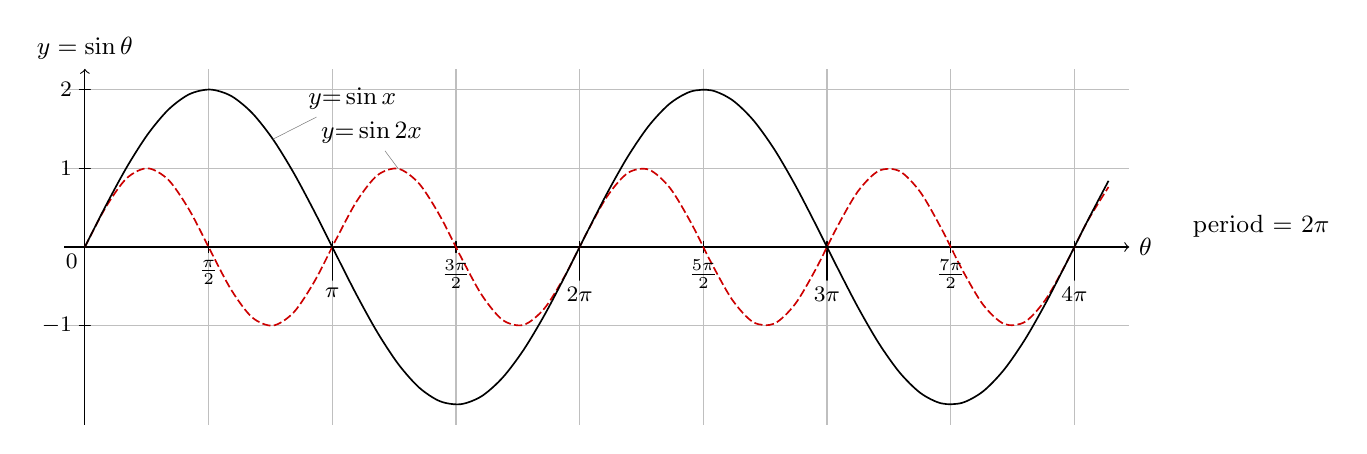
\begin{tikzpicture}
  \datavisualization [ school book axes,
  all axes={grid, unit length=1.0cm},
  y axis={label={$y=\sin\theta$}},
  x axis={label={$\theta$}},
  x axis={ticks=stack, ticks and grid={major={at={
          (pi/2) as $\frac{\pi}{2}$,
          (pi) as $\pi$,
          (3*pi/2) as $\frac{3\pi}{2}$,
          (2*pi) as $2\pi$,
          (5*pi/2) as $\frac{5\pi}{2}$,
          (3*pi) as $3\pi$,
          (7*pi/2) as $\frac{7\pi}{2}$,
          (4*pi) as $4\pi$
        }}}},
  visualize as smooth line/.list={sinx,sin2x},
  style sheet=strong colors,
  style sheet=vary dashing,
  sinx={pin in data={text=$y \text{=} \sin x$, when=x is (3*pi/4)}},
  sin2x={pin in data={text=$y \text{=} \sin 2x$, when=x is (5*pi/4), pin angle=30}},
  new legend entry={text=\text{period =} $2\pi$},
  data/format=function ]
  data [set=sinx] {
    var x : interval [0:13] samples 50;
    func y = 2*sin(\value x r);
  }
  data [set=sin2x] {
    var x : interval [0:13] samples 50;
    func y = sin(\value x*2 r);
  };
\end{tikzpicture}

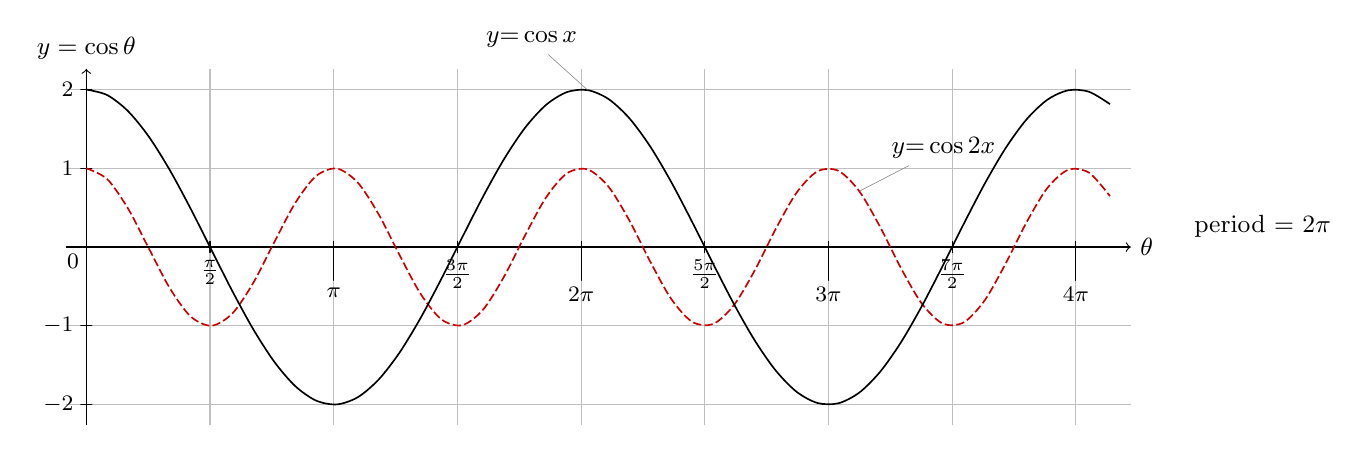
\begin{tikzpicture}
  \datavisualization [ school book axes,
  all axes={grid, unit length=1.0cm},
  y axis={label={$y=\cos\theta$}},
  x axis={label={$\theta$}},
  x axis={ticks=stack, ticks and grid={major={at={
          (pi/2) as $\frac{\pi}{2}$,
          (pi) as $\pi$,
          (3*pi/2) as $\frac{3\pi}{2}$,
          (2*pi) as $2\pi$,
          (5*pi/2) as $\frac{5\pi}{2}$,
          (3*pi) as $3\pi$,
          (7*pi/2) as $\frac{7\pi}{2}$,
          (4*pi) as $4\pi$
        }}}},
  visualize as smooth line/.list={cosx,cos2x},
  style sheet=strong colors,
  style sheet=vary dashing,
  cosx={pin in data={text=$y \text{=} \cos x$, when=x is (2*pi)}},
  cos2x={pin in data={text=$y \text{=} \cos 2x$}},
  new legend entry={text=\text{period =} $2\pi$},
  data/format=function ]
  data [set=cosx] {
    var x : interval [0:13] samples 50;
    func y = 2*cos(\value x r);
  }
  data [set=cos2x] {
    var x : interval [0:13] samples 50;
    func y = cos(\value x*2 r);
  };
\end{tikzpicture}

\paragraph{Example 1.}

Find the period of

\begin{enumerate*}[label=\roman*)]
  \item $\cos \frac{x}{2} = 4\pi$
  \item $\cos 2x = \pi$
  \item $\cos \frac{x}{3} = 6\pi$
  \item $\cos 3x = \frac{2\pi}{3}$
  \item $\cos \frac{1}{2} (x+2) = 4\pi$
  \item $3\cos4x+1 = \frac{\pi}{2}$
\end{enumerate*}

\paragraph{Example 2.}

Find the basic sine function whose period is

\begin{enumerate*}[label=\roman*)]
  \item $\frac{\pi}{5} \Rightarrow \sin 10x$
  \item $6\pi \Rightarrow \sin \frac{x}{3}$
  \item $\frac{\pi}{4} \Rightarrow \sin 8x$
\end{enumerate*}

\paragraph{Example 3.}

Solve

\begin{enumerate}[label=\alph*)]
  \item What is the maximum and minimum value of function $y = 2\sin x + 3$

        {\scriptsize \textbf{Solution:}}
        Min = $1$, Max = $5$ as $\sin x$ has max value of $1$ and min value of $-1$.

  \item What is the maximum and minimum value of function $y = 3\cos x - 2$

        {\scriptsize \textbf{Solution:}}
        Min = $-5$, Max = $1$
\end{enumerate}

\paragraph{Example 4.}

If $\cos x = \frac{-1}{2}$, find the exact solution where $0 \leq x \leq 4\pi$

{\scriptsize \textbf{Solution:}}
\[
  \begin{aligned}
    x = \frac{2\pi}{3}, \frac{4\pi}{3}, \frac{8\pi}{3}, \frac{10\pi}{3}
  \end{aligned}
\]

\paragraph{Example 5.}

If $\sin x = \frac{1}{2}$, find the exact solution where $0 \leq x \leq 540^{\circ}$

{\scriptsize \textbf{Solution:}}
\[
  \begin{aligned}
    x = 30^{\circ}, 150^{\circ}, 390^{\circ}, 510^{\circ}
  \end{aligned}
\]

\paragraph{Example 6.}

If $\tan x = \sqrt{3}$, find the exact solution where $0 \leq x \leq 540^{\circ}$

{\scriptsize \textbf{Solution:}}
\[
  \begin{aligned}
    x = 60^{\circ}, 240^{\circ}, 420^{\circ}
  \end{aligned}
\]

\paragraph{Example 7.}

Solve for $x$, $\tan(x-\frac{\pi}{3}) = 1$, where $0 \leq x \leq 3\pi$

{\scriptsize \textbf{Solution:}}
\[
  \begin{aligned}
    \tan(x-\frac{\pi}{3}) = 1 \\
    x - \frac{\pi}{3} = \frac{\pi}{4}, \frac{5\pi}{4}, \frac{9\pi}{4} \\
    x = \frac{7\pi}{12}, \frac{19\pi}{12}, \frac{31\pi}{12}
  \end{aligned}
\]

\paragraph{Example 8.}

Solve for $x$, $\cos(x-\frac{\pi}{3}) = \frac{1}{2}$, where $0 \leq x \leq 4\pi$

{\scriptsize \textbf{Solution:}}
\[
  \begin{aligned}
    \cos(x-\frac{\pi}{3}) = \frac{1}{2} \\
    x - \frac{\pi}{3} = \frac{\pi}{4}, \frac{5\pi}{4}, \frac{9\pi}{4} \\
    x - \frac{\pi}{3} = \left. \begin{array}{c} \pi/3 \\ 5\pi/3 \end{array} \right\} + 2K\pi, \text{where } K = 0, 1, 2 \\
    x = \left. \begin{array}{c} 2\pi/3 \\ 2\pi \end{array} \right\} + 2\pi or + 3\pi \\
    x = \frac{2\pi}{3}, 2\pi, \frac{8\pi}{3}, 4\pi
  \end{aligned}
\]

\paragraph{Generation equation}
\[ y = A \sin(B(x + C)) + D \] where $A$ = amplitude, $B$ = effective period, $C$ = transition to left along $x$ axis, $D$ = vertical transition, if $C$ is negative, then transition to right along $x$ axis.

\subsection {Exercise 18.4}
\paragraph{Q1.}
Draw the graph of $y=\cos\theta, 0 \leq \theta \leq 720^{\circ}$.
Read and write the values of $\theta$ for which $\cos\theta$ equals

\begin{enumerate*}[label=\alph*)]
  \item $\frac{-1}{2}$
  \item $\frac{1}{2}$
  \item $1$
  \item $0$
\end{enumerate*}

\paragraph{Q2.}
Draw the graph of $f(x)=\sin 2x, -2\pi \leq x \leq 4\pi$

\paragraph{Q3.}
Draw the graph of $y=\cos 2x, 0 \leq x \leq 2\pi$

\paragraph{Q4.}
Draw the graph of $y=\cos(x+\frac{\pi}{3}), -2\pi \leq x \leq 4\pi$

\paragraph{Q5.}
Draw the graph of $y=\sin x, 0 \leq x \leq 720^{\circ}$.
Read from the graph and write the values of $x$ for which $\sin\theta$ equals

\begin{enumerate*}[label=\alph*)]
  \item $1$
  \item $\frac{1}{2}$
  \item $\frac{\sqrt{3}}{2}$
  \item $0$
  \item $-1$
  \item $\frac{-1}{2}$
\end{enumerate*}

\paragraph{Q6.}
Complete the table

\begin{tabular}{|c|c|c|c|c|c|c|c|c|c|c|c|c|c|}
  \hline
$\theta$ & $0$ & $\frac{\pi}{6}$ & $\frac{2\pi}{6}$ & $\frac{3\pi}{6}$ & $\frac{4\pi}{6}$ & $\frac{5\pi}{6}$ & $\pi$ & $\frac{7\pi}{6}$ & $\frac{8\pi}{6}$ & $\frac{9\pi}{6}$ & $\frac{10\pi}{6}$ & $\frac{11\pi}{6}$ & $2\pi$ \\[3pt]
  \hline
$\sin\theta$ & $0$ & & & & & & & & & & & &\\
  \hline
\end{tabular}

\paragraph{Q7.}
Draw graph of $y = \cos \frac{x}{2}$.

\begin{enumerate*}[label=\alph*)]
  \item Find zeros of $y = \cos \frac{x}{2} = 0$
  \item Find $x$ where $\cos \frac{x}{2} = \frac{1}{2}$
  \item Find $x$ where $\cos \frac{x}{2} = \frac{-1}{2}$
\end{enumerate*}

\paragraph{Q8.}
Draw graph of $y = 2\cos x$.

\paragraph{Q9.}
Draw graph of $y = \frac{1}{3} \sin x$.

\paragraph{Q10.}
Draw graph of $y = - \cos x$.

\paragraph{Q11.}
Draw graph of $y = \sin (-x)$.

\subsubsection {Answers to Exercise 18.4}

\paragraph{Q1.}
Graph

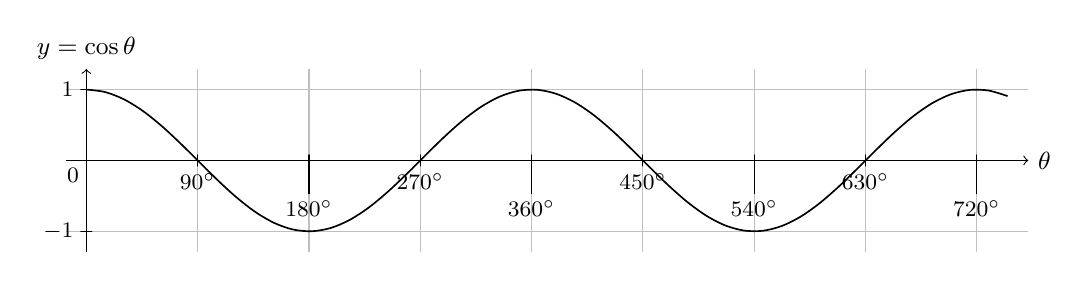
\begin{tikzpicture}
  \datavisualization [ school book axes,
  all axes={grid, unit length=0.9cm},
  y axis={label={$y=\cos\theta$}},
  x axis={label={$\theta$}},
  x axis={ticks=stack, ticks and grid={major={at={
          (pi/2) as $90^{\circ}$,
          (pi) as $180^{\circ}$,
          (3*pi/2) as $270^{\circ}$,
          (2*pi) as $360^{\circ}$,
          (5*pi/2) as $450^{\circ}$,
          (3*pi) as $540^{\circ}$,
          (7*pi/2) as $630^{\circ}$,
          (4*pi) as $720^{\circ}$
        }}}},
  visualize as smooth line/.list={cosx},
  style sheet=strong colors,
  data/format=function ]
  data [set=cosx] {
    var x : interval [0:13] samples 50;
    func y = cos(\value x r);
  };
\end{tikzpicture}

\begin{enumerate*}[label=\alph*)]
          \item $120^{\circ}, 240^{\circ}, 480^{\circ}, 600^{\circ}$
          \item $60^{\circ}, 300^{\circ}, 420^{\circ}, 660^{\circ}$
          \item $180^{\circ}, 540^{\circ}$
          \item $90^{\circ}, 270^{\circ}, 450^{\circ}, 630^{\circ}$
\end{enumerate*}


\paragraph{Q2.}
The value of $n$ is $2$, so the period is $\tau = \frac{2\pi}{n} = \frac{2\pi}{2} = \pi$. Note that this means the period is \textbf{half} that of the basic sine function.

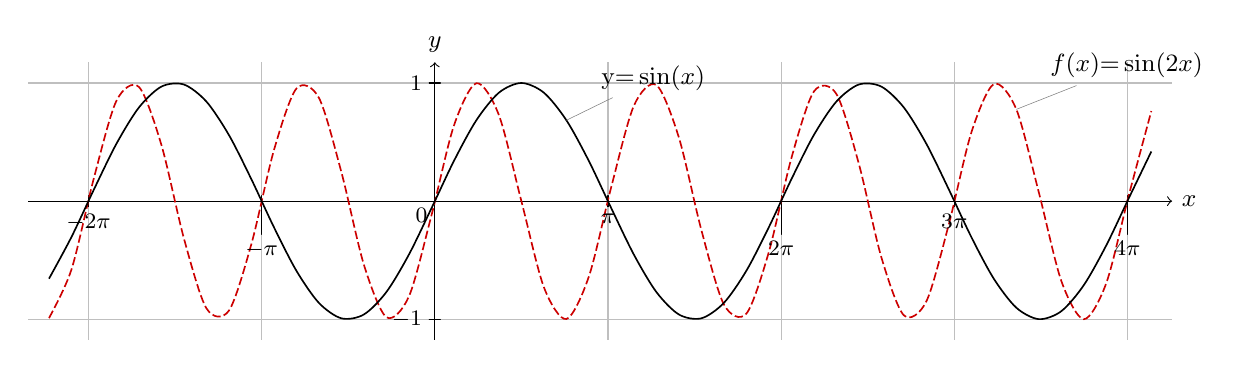
\begin{tikzpicture}
  \datavisualization [ school book axes,
  all axes={grid, unit length=0.7cm},
  y axis={length=3cm, label={$y$}},
  x axis={include value=-7},
  x axis={label={$x$}},
  x axis={ticks=stack, ticks and grid={major={at={
          (-2*pi) as $-2\pi$,
          (-pi) as $-\pi$,
          (pi) as $\pi$,
          (2*pi) as $2\pi$,
          (3*pi) as $3\pi$,
          (4*pi) as $4\pi$
        }}}},
  visualize as smooth line/.list={sinx,sin2x},
  style sheet=strong colors,
  style sheet=vary dashing,
  sinx={pin in data={text=$\text{y=}\sin (x)$, when=x is (1.3*pi/2)}},
  sin2x={pin in data={text=$f(x)\text{=}\sin (2x)$, when=x is (13*pi/4)}},
  data/format=function ]
  data [set=sinx] {
    var x : interval [-7:13] samples 50;
    func y = sin(\value x r);
  }
  data [set=sin2x] {
    var x : interval [-7:13] samples 50;
    func y = sin(\value x*2 r);
  };
\end{tikzpicture}

\paragraph{Q3.}
Graph

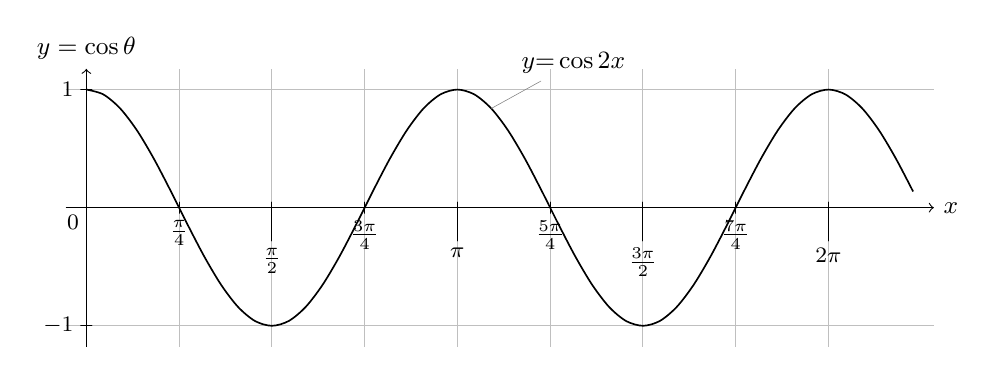
\begin{tikzpicture}
  \datavisualization [ school book axes,
  all axes={grid, unit length=1.5cm},
  y axis={label={$y=\cos\theta$}},
  x axis={label={$x$}},
  x axis={ticks=stack, ticks and grid={major at={
          (pi/4) as $\frac{\pi}{4}$,
          (pi/2) as $\frac{\pi}{2}$,
          (3*pi/4) as $\frac{3\pi}{4}$,
          (pi) as $\pi$,
          (5*pi/4) as $\frac{5\pi}{4}$,
          (3*pi/2) as $\frac{3\pi}{2}$,
          (7*pi/4) as $\frac{7\pi}{4}$,
          (2*pi) as $2\pi$
        }}},
  visualize as smooth line/.list={cos2x},
  style sheet=strong colors,
  style sheet=vary dashing,
  cos2x={pin in data={text=$y \text{=} \cos 2x$}},
  data/format=function ]
  data [set=cos2x] {
    var x : interval [0:7] samples 50;
    func y = cos(\value x*2 r);
  };
\end{tikzpicture}

\paragraph{Q4.}
Basic cosine graph when translated $\frac{\pi}{3}$ units to the left.

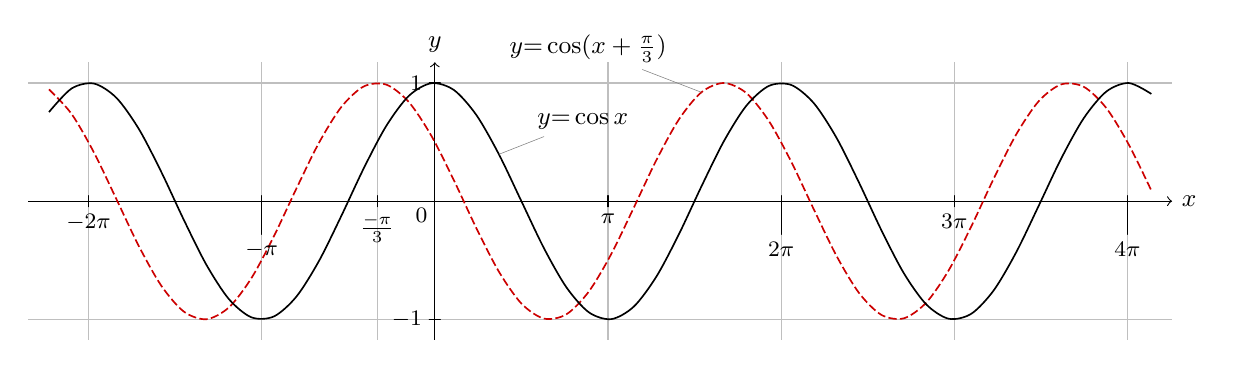
\begin{tikzpicture}
  \datavisualization [ school book axes,
  all axes={grid, unit length=0.7cm},
  y axis={length=3cm, label={$y$}},
  x axis={label={$x$}},
  x axis={ticks=stack, ticks and grid={major at={
          (-2*pi) as $-2\pi$,
          (-pi) as $-\pi$,
          (pi) as $\pi$,
          (2*pi) as $2\pi$,
          (3*pi) as $3\pi$,
          (4*pi) as $4\pi$
        }}},
  x axis={ticks and grid={major also at={
          (-pi/3) as $\frac{-\pi}{3}$
        }}},
  visualize as smooth line/.list={cosx, cosc},
  style sheet=strong colors,
  style sheet=vary dashing,
  cosx={pin in data={text=$y \text{=} \cos x$, when=x is (pi/4)}},
  cosc={pin in data={text=$y \text{=} \cos (x + \frac{\pi}{3})$, when=x is (3*pi/2)}},
  data/format=function ]
  data [set=cosx] {
    var x : interval [-7:13] samples 50;
    func y = cos(\value x r);
  }
  data [set=cosc] {
    var c : {1.0471975512};
    var x : interval [-7:13] samples 50;
    func y = cos((\value x + \value c) r);
  };
\end{tikzpicture}

\paragraph{Q5.}
Graph

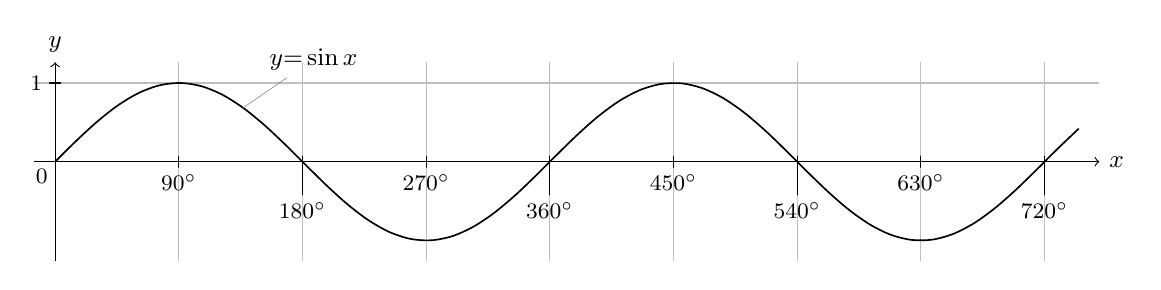
\begin{tikzpicture}
  \datavisualization [ school book axes,
  all axes={grid, unit length=1.0cm},
  y axis={label={$y$}},
  x axis={label={$x$}},
  x axis={ticks=stack, ticks and grid={major={at={
          (pi/2) as $90^{\circ}$,
          (pi) as $180^{\circ}$,
          (3*pi/2) as $270^{\circ}$,
          (2*pi) as $360^{\circ}$,
          (5*pi/2) as $450^{\circ}$,
          (3*pi) as $540^{\circ}$,
          (7*pi/2) as $630^{\circ}$,
          (4*pi) as $720^{\circ}$
        }}}},
  visualize as smooth line/.list={sinx},
  style sheet=strong colors,
  sinx={pin in data={text=$y \text{=} \sin x$, when=x is (3*pi/4)}},
  data/format=function ]
  data [set=sinx] {
    var x : interval [0:13] samples 50;
    func y = sin(\value x r);
  };
\end{tikzpicture}

\begin{enumerate*}[label=\alph*)]
          \item $90^{\circ}, 450^{\circ}$
          \item $30^{\circ}, 150^{\circ}, 390^{\circ}, 510^{\circ}$
          \item $60^{\circ}, 120^{\circ}, 420^{\circ}, 480^{\circ}$
          \item $180^{\circ}, 360^{\circ}, 540^{\circ}, 720^{\circ}$
          \item $270^{\circ}, 630^{\circ}$
          \item $210^{\circ}, 330^{\circ}, 570^{\circ}, 690^{\circ}$
\end{enumerate*}

\paragraph{Q6.}
Complete the table

\begin{tabular}{|c|c|c|c|c|c|c|c|c|c|c|c|c|c|}
  \hline
$\theta$ & $0$ & $\frac{\pi}{6}$ & $\frac{2\pi}{6}$ & $\frac{3\pi}{6}$ & $\frac{4\pi}{6}$ & $\frac{5\pi}{6}$ & $\pi$ & $\frac{7\pi}{6}$ & $\frac{8\pi}{6}$ & $\frac{9\pi}{6}$ & $\frac{10\pi}{6}$ & $\frac{11\pi}{6}$ & $2\pi$ \\[3pt]
  \hline
$\sin\theta$ & $0$ & $\frac{1}{2}$ & $\frac{\sqrt{3}}{2}$ & $1$ & $\frac{\sqrt{3}}{2}$ & $\frac{1}{2}$ & $0$ & $\frac{-1}{2}$ & $\frac{-\sqrt{3}}{2}$ & $-1$ & $\frac{-\sqrt{3}}{2}$ & $\frac{-1}{2}$ & $0$ \\
  \hline
\end{tabular}

\paragraph{Q7.}
$f(x) = \cos(\frac{x}{2})$, in this case the value of $n = \frac{1}{2}$ and the period $\tau = \frac{2\pi}{n} = \frac{2\pi}{1/2} = 4\pi$

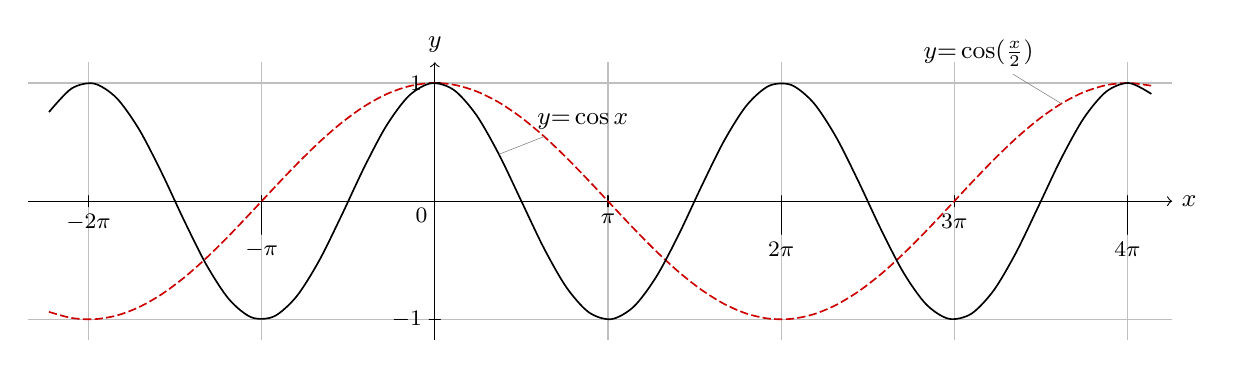
\begin{tikzpicture}
  \datavisualization [ school book axes,
  all axes={grid, unit length=0.7cm},
  y axis={length=3cm, label={$y$}},
  x axis={label={$x$}},
  x axis={ticks=stack, ticks and grid={major at={
          (-2*pi) as $-2\pi$,
          (-pi) as $-\pi$,
          (pi) as $\pi$,
          (2*pi) as $2\pi$,
          (3*pi) as $3\pi$,
          (4*pi) as $4\pi$
        }}},
  visualize as smooth line/.list={cosx, cosc},
  style sheet=strong colors,
  style sheet=vary dashing,
  cosx={pin in data={text=$y \text{=} \cos x$, when=x is (pi/4)}},
  cosc={pin in data={text=$y \text{=} \cos (\frac{x}{2})$, when=x is (7*pi/2)}},
  data/format=function ]
  data [set=cosx] {
    var x : interval [-7:13] samples 50;
    func y = cos(\value x r);
  }
  data [set=cosc] {
    var x : interval [-7:13] samples 50;
    func y = cos((\value x / 2) r);
  };
\end{tikzpicture}

\begin{enumerate}[label=\alph*)]
  \item Zeros of $y=\cos(x/2)$, $x = -3\pi, -\pi, \pi, 3\pi, 5\pi$
  \item $\cos \frac{x}{2} = \frac{1}{2}$ $\therefore x = 0, 4\pi$
  \item $\cos \frac{x}{2} = \frac{-1}{2}$ $\therefore x = 2\pi$
\end{enumerate}

\paragraph{Q8.}
The cosine graph with an amplitude of $2$.

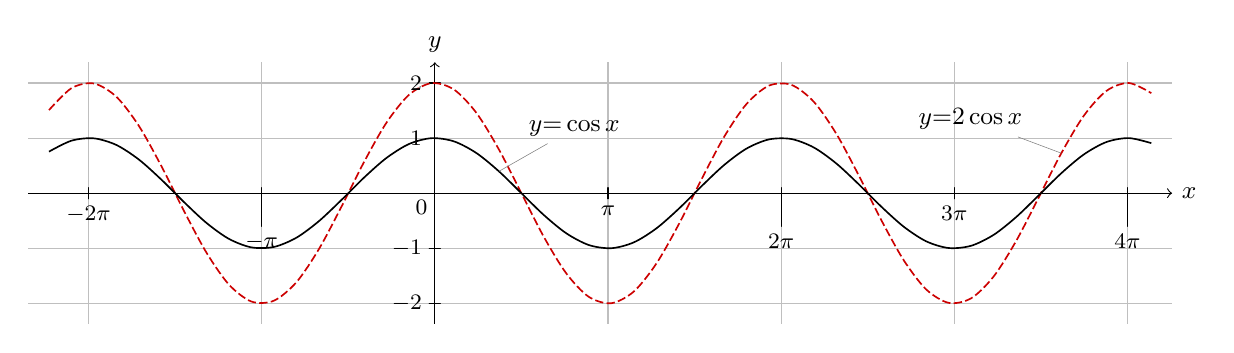
\begin{tikzpicture}
  \datavisualization [ school book axes,
  all axes={grid, unit length=0.7cm},
  y axis={label={$y$}},
  x axis={label={$x$}},
  x axis={ticks=stack, ticks and grid={major at={
          (-2*pi) as $-2\pi$,
          (-pi) as $-\pi$,
          (pi) as $\pi$,
          (2*pi) as $2\pi$,
          (3*pi) as $3\pi$,
          (4*pi) as $4\pi$
        }}},
  visualize as smooth line/.list={cosx, cosc},
  style sheet=strong colors,
  style sheet=vary dashing,
  cosx={pin in data={text=$y \text{=} \cos x$, when=x is (pi/4)}},
  cosc={pin in data={text=$y \text{=} 2 \cos x$, when=x is (7*pi/2)}},
  data/format=function ]
  data [set=cosx] {
    var x : interval [-7:13] samples 50;
    func y = cos(\value x r);
  }
  data [set=cosc] {
    var x : interval [-7:13] samples 50;
    func y = 2 * cos(\value x r);
  };
\end{tikzpicture}

\paragraph{Q9.}
The cosine graph with an amplitude of $\frac{1}{3}$.

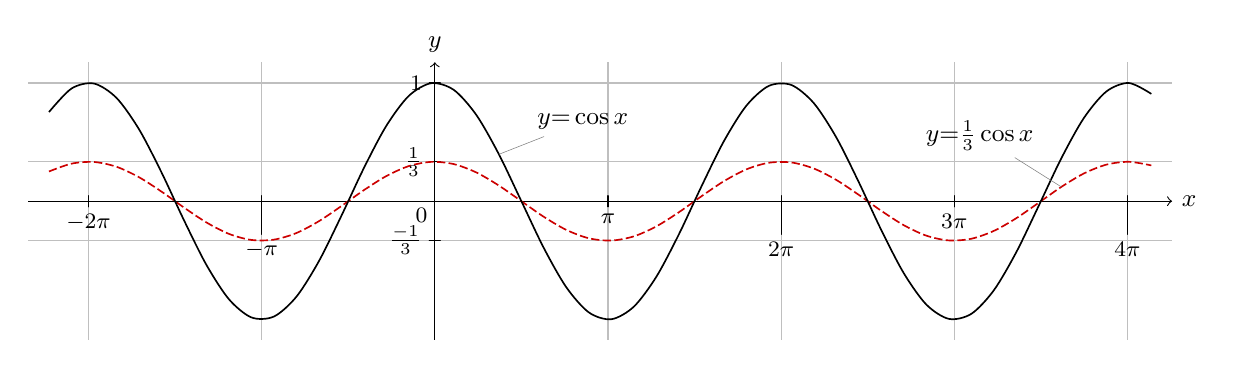
\begin{tikzpicture}
  \datavisualization [ school book axes,
  all axes={grid, unit length=0.7cm},
  y axis={length=3cm, label={$y$}},
  y axis={ticks and grid={major also at={
        (1/3) as $\frac{1}{3}$,
        (-1/3) as $\frac{-1}{3}$
        }}},
  x axis={label={$x$}},
  x axis={ticks=stack, ticks and grid={major at={
          (-2*pi) as $-2\pi$,
          (-pi) as $-\pi$,
          (pi) as $\pi$,
          (2*pi) as $2\pi$,
          (3*pi) as $3\pi$,
          (4*pi) as $4\pi$
        }}},
  visualize as smooth line/.list={cosx, cosc},
  style sheet=strong colors,
  style sheet=vary dashing,
  cosx={pin in data={text=$y \text{=} \cos x$, when=x is (pi/4)}},
  cosc={pin in data={text=$y \text{=} \frac{1}{3} \cos x$, when=x is (7*pi/2)}},
  data/format=function ]
  data [set=cosx] {
    var x : interval [-7:13] samples 50;
    func y = cos(\value x r);
  }
  data [set=cosc] {
    var x : interval [-7:13] samples 50;
    func y = 1/3 * cos(\value x r);
  };
\end{tikzpicture}

\paragraph{Q10.}
Basic cosine graph when $f(x) = -\cos(x)$.

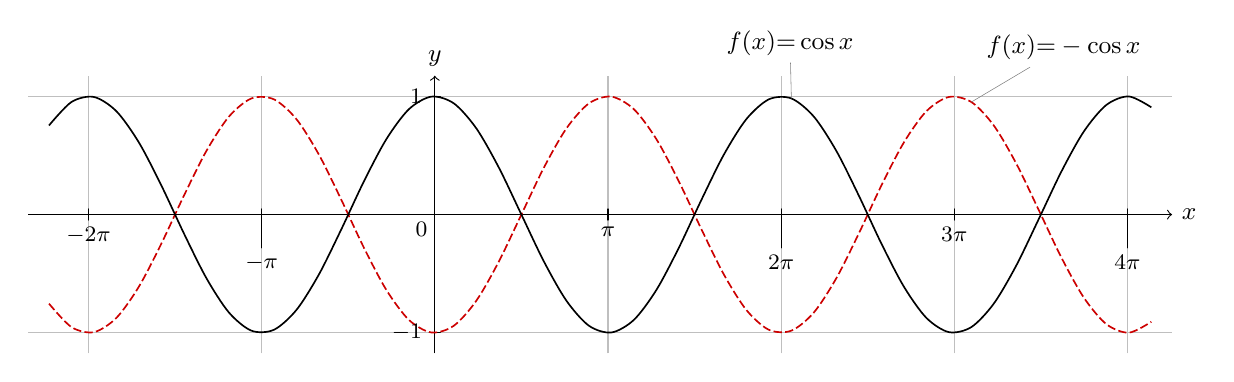
\begin{tikzpicture}
  \datavisualization [ school book axes,
  all axes={grid, unit length=0.7cm},
  y axis={length=3cm, label={$y$}},
  x axis={label={$x$}},
  x axis={ticks=stack, ticks and grid={major at={
          (-2*pi) as $-2\pi$,
          (-pi) as $-\pi$,
          (pi) as $\pi$,
          (2*pi) as $2\pi$,
          (3*pi) as $3\pi$,
          (4*pi) as $4\pi$
        }}},
  visualize as smooth line/.list={cosx, cosc},
  style sheet=strong colors,
  style sheet=vary dashing,
  cosx={pin in data={text=$f(x) \text{=} \cos x$, when=x is (2*pi)}},
  cosc={pin in data={text=$f(x) \text{=} - \cos x$, when=x is (3*pi)}},
  data/format=function ]
  data [set=cosx] {
    var x : interval [-7:13] samples 50;
    func y = cos(\value x r);
  }
  data [set=cosc] {
    var x : interval [-7:13] samples 50;
    func y = -cos(\value x r);
  };
\end{tikzpicture}

\paragraph{Q11.}
Basic sine graph when $f(x) = \sin(-x)$.

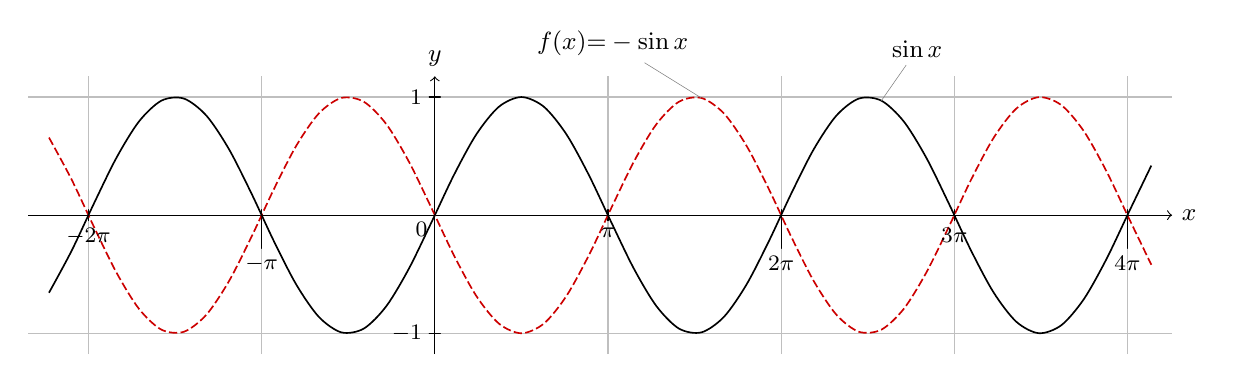
\begin{tikzpicture}
  \datavisualization [ school book axes,
  all axes={grid, unit length=0.7cm},
  y axis={length=3cm, label={$y$}},
  x axis={label={$x$}},
  x axis={ticks=stack, ticks and grid={major at={
          (-2*pi) as $-2\pi$,
          (-pi) as $-\pi$,
          (pi) as $\pi$,
          (2*pi) as $2\pi$,
          (3*pi) as $3\pi$,
          (4*pi) as $4\pi$
        }}},
  visualize as smooth line/.list={sinx, sinc},
  style sheet=strong colors,
  style sheet=vary dashing,
  sinx={pin in data={text=$\sin x$, when=x is (5*pi/2)}},
  sinc={pin in data={text=$f(x) \text{=} -\sin x$, when=x is (3*pi/2)}},
  data/format=function ]
  data [set=sinx] {
    var x : interval [-7:13] samples 50;
    func y = sin(\value x r);
  }
  data [set=sinc] {
    var x : interval [-7:13] samples 50;
    func y = -sin(\value x r);
  };
\end{tikzpicture}

\subsubsection {Solve trigonometric equations.}

\paragraph{Example 1.}
\textbf{Solve:} $2\cos^{2}x - \sin x + 1=0, 0 \leq x \leq 2\pi$

{\scriptsize \textbf{Solution:}}
\[
  \begin{aligned}
    2(1 - \sin^{2}x) - \sin x + 1 = 0 \\
    2\sin^{2}x + \sin x - 1 = 0 \Rightarrow 2\sin^{2}x + 2\sin x - \sin x - 1 = 0 \\
    (2\sin x - 1)(\sin x + 1) = 0 \\
    \sin x = \frac{1}{2} \Rightarrow \frac{\pi}{6}, \frac{5\pi}{6} \\
    \sin x = 1 \Rightarrow \frac{3\pi}{2} \\
    x = \frac{\pi}{6}, \frac{3\pi}{2}, \frac{5\pi}{6}
  \end{aligned}
\]

\paragraph{Example 2.}
\textbf{Solve:} $2\sin^{2}x = \sin x, 0 < x < 2\pi$

{\scriptsize \textbf{Solution:}}
\[
  \begin{aligned}
    2\sin^{2}x = \sin x \\
    \sin x(2\sin^{2}x - 1) = 0 \\
    \sin x = 0 \Rightarrow 0, \pi, 2\pi \\
    \sin x = \frac{1}{2} \Rightarrow \frac{\pi}{6}, \frac{5\pi}{6} \\
    x = 0, \frac{\pi}{6}, \frac{5\pi}{6}, \pi, 2\pi
  \end{aligned}
\]

\paragraph{Example 3.}
\textbf{Solve:} $2\cos^{2}x = \cos x, 0 < x \leq 2\pi$

{\scriptsize \textbf{Solution:}}
\[
  \begin{aligned}
    2\cos^{2}x = \cos x \\
    \cos x(2\cos^{2}x - 1) = 0 \\
    \cos x = 0 \Rightarrow \frac{\pi}{2}, \frac{3\pi}{2} \\
    \cos x = \frac{1}{2} \Rightarrow \frac{\pi}{3}, \frac{11\pi}{6} \\
    x = \frac{\pi}{3}, \frac{\pi}{2}, \frac{3\pi}{2}, \frac{11\pi}{6}
  \end{aligned}
\]

\paragraph{Example 4.}
\textbf{Solve:} $2\sin^{2}x - \cos x - 1=0, 0 \leq x \leq 2\pi$

{\scriptsize \textbf{Solution:}}
\[
  \begin{aligned}
    2(1 - \cos^{2}x) - \cos x - 1 = 0 \\
    2\cos^{2}x - 2 \cos x + \cos x - 1 = 0 \\
    2\cos x(\cos x - 1) + 1 (\cos x - 1) = 0 \\
    (2\cos x + 1) (\cos x - 1) = 0 \\
    \cos x = \frac{-1}{2} \Rightarrow x = \frac{2\pi}{3}, \frac{4\pi}{3} \\
    \cos x = 1 \Rightarrow x = 0, 2\pi
  \end{aligned}
\]

\paragraph{Example 5.}
\textbf{Solve:} $2\sec^{2}\theta - 5\tan\theta - 5=0, 0 \leq \theta \leq 2\pi$

{\scriptsize \textbf{Solution:}}
\[
  \begin{aligned}
    2\sec^{2}\theta - 5\tan\theta - 5=0 \\
    2(1+\tan^{2}\theta) - 5\tan\theta - 5 = 0 \\
    2\tan^{2}\theta - 5\tan\theta - 3 = 0 \\
    2\tan^{2}\theta - 6\tan\theta + \tan\theta - 3 = 0 \\
    2\tan^{2}\theta(\tan\theta - 3) + 1(\tan\theta-3) = 0 \\
    (2\tan\theta+1)(\tan\theta-3)=0 \\
    \tan\theta = \frac{-1}{2} \\
    \tan\theta = 3
  \end{aligned}
\]

\paragraph{Example 6.}
\textbf{Solve:} $2\sin^{2}x - 3\sin x + 1=0, 0^{\circ} < 0 \leq 360^{\circ}$

{\scriptsize \textbf{Solution:}}
\[
  \begin{aligned}
    2\sin^{2}x - 3\sin x + 1=0 \\
    2\sin^{2}x - 2\sin x - \sin x + 1 = 0 \\
    2\sin x(\sin x - 1) - 1(\sin x - 1) = 0 \\
    (2\sin x - 1)(\sin x - 1) = 0 \\
    \sin x = \frac{1}{2} \Rightarrow x = \frac{\pi}{6}, \frac{5\pi}{6} \\
    OR \sin x = 1 \Rightarrow x = \frac{\pi}{2} \\
    x = \frac{\pi}{6}, \frac{\pi}{2}, \frac{5\pi}{6}
  \end{aligned}
\]

\paragraph{Example 7.}
\textbf{Solve:} $\tan\theta + \cot\theta=2, 0 \leq \theta \leq 2\pi$

{\scriptsize \textbf{Solution:}}
\[
  \begin{aligned}
    \tan\theta + \cot\theta=2 \\
    \tan\theta + \frac{1}{\tan\theta}=2 \\
    \tan^{2}\theta - 2 \tan\theta + 1=0 \\
    (\tan\theta - 1)^{2}=0 \\
    \tan\theta =1 \Rightarrow \theta = \frac{\pi}{4}, \frac{5\pi}{4}
  \end{aligned}
\]

\paragraph{Example 8.}
\textbf{Solve:} $\sin^{2}\theta - 2\cos\theta + \frac{1}{4}=0$

{\scriptsize \textbf{Solution:}}
\[
  \begin{aligned}
    \sin^{2}\theta - 2\cos\theta + \frac{1}{4}=0 \\
    1 - \cos^{2}\theta - 2\cos\theta + \frac{1}{4}=0 \\
    4\cos^{2}\theta + 8\cos\theta - 5=0 \\
    4\cos^{2}\theta + 10\cos\theta - 2\cos\theta - 5=0 \\
    2\cos\theta(2\cos\theta+5) - 1(2\cos\theta + 5)=0 \\
    (2\cos\theta-1)(2\cos\theta + 5)=0 \\
    \cos\theta=\frac{1}{2} \Rightarrow \theta = \frac{\pi}{3}, \frac{5\pi}{3} \\
    \cos\theta=\frac{-5}{2} \text{ which is not admissible}
  \end{aligned}
\]

\paragraph{Example 9.}
\textbf{Solve:} $\cos\theta = 1 + \sqrt{3}\sin\theta, 0 \leq \theta \leq 2\pi$

{\scriptsize \textbf{Solution:}}
\[
  \begin{aligned}
    \cos\theta = 1 + \sqrt{3}\sin\theta \\
    \cos^{2}\theta = 1 +3\sin^{2}\theta + 2 \sqrt{3}\sin\theta \\
    1 - \sin^{2}\theta = 1 +3\sin^{2}\theta + 2 \sqrt{3}\sin\theta \\
    2 \sin\theta(2\sin\theta + \sqrt{3}) = 0 \\
    \sin\theta = 0 \Rightarrow \theta = 0, \pi, 2\pi \\
    \sin\theta = \frac{-\sqrt{3}}{2} \Rightarrow \theta = \frac{4\pi}{3}, \frac{5\pi}{3}
  \end{aligned}
\]

\paragraph{Example 10.}
\textbf{Solve:} $\sin\theta + 2\cos\theta = 1, 0 \leq \theta \leq 2\pi$

{\scriptsize \textbf{Solution:}}
\[
  \begin{aligned}
    \sin\theta + 2\cos\theta = 1 \\
    (2\cos\theta)^{2} = (1 -\sin\theta)^{2} \\
    4\cos^{2}\theta = 1 +\sin^{2}\theta - 2\sin\theta \\
    4(1-\sin^{2}\theta) = 1 +\sin^{2}\theta - 2\sin\theta \\
    5\sin^{2}\theta - 2\sin\theta - 3 = 0 \\
    5\sin^{2}\theta - 5\sin\theta + 3\sin\theta - 3 = 0 \\
    (5\sin\theta+3)(\sin\theta-1)= 0 \\
    \sin\theta = 1, \Rightarrow \theta = \frac{\pi}{2} \\
    \sin\theta = \frac{-3}{5} \Rightarrow \theta = \sin^{-1}0.6
  \end{aligned}
\]

\subsection {Exercise 18.5}
\paragraph{Solve for $\theta$}

\begin{enumerate}[label=Q\arabic*)]
  \item $6\sin^{2}\theta + 13\sin\theta + 5 = 0, 0 \leq x \leq 2\pi$
  \item $6\sin^{2}\theta + 5\sin\theta - 4 = 0, 0 \leq \theta \leq 2\pi$
  \item $4\cos^{2}\theta + 4\cos\theta - 3 = 0, 0 \leq \theta \leq 2\pi$
  \item $4\sin^{2}\theta + 12\sin\theta + 5 = 0, 0 \leq \theta \leq 2\pi$
  \item $6\cos^{2}\theta - \cos\theta - 2 = 0, 0 \leq \theta \leq 2\pi$
  \item $\frac{14}{\sin\theta+3} - 1 = \frac{5}{\sin\theta+1}, 0 \leq \theta \leq 2\pi$
  \item $\frac{\sin x+3}{\sin x+2} = \frac{3\sin x-7}{2\sin x-3}, 0 \leq \theta \leq 2\pi$
  \item $\frac{1}{\cos\theta+4} - \frac{1}{\cos\theta-7} = \frac{11}{30}, 0 \leq \theta \leq 2\pi$
  \item $3\sin^{2}\theta + 2\cos\theta + 2 = 0, 0 \leq \theta \leq 2\pi$
\end{enumerate}

\subsubsection {Answers to Exercise 18.5}

\begin{enumerate*}[label=Q\arabic*)]
  \item $\frac{7\pi}{6}, \frac{11\pi}{6}$
  \item $\frac{\pi}{6}, \frac{5\pi}{6}$
  \item $\frac{\pi}{3}, \frac{5\pi}{3}$
  \item $\frac{\pi}{3}, \frac{5\pi}{3}$
  \item $\frac{7\pi}{6}, \frac{11\pi}{6}$
  \item $\frac{2\pi}{3}, \frac{4\pi}{3}$
  \item $\frac{\pi}{2}$
  \item $\frac{3\pi}{2}$
  \item $0, 2\pi$
  \item $0, 1.911, 4.373 \text{ or } 6.283$
\end{enumerate*}

\subsection{Opposite real number identities}

\begin{enumerate}
        \begin{paracol}{2}
          \item $\sin(-\theta) = -\sin\theta$
          \item $\cos(-\theta) = \cos\theta$
          \item $\tan(-\theta) = -\tan\theta$
          \switchcolumn
          \item[4.] $\cos(90-\theta) = \sin\theta$
          \item[5.] $\sin(90-\theta) = \cos\theta$
          \item[6.] $\tan(90-\theta) = \cot\theta$
        \end{paracol}
\end{enumerate}

\paragraph{Example 1.}
Simplify

\begin{enumerate*}[label=\alph*)]
  \item $5\sin\theta - 2\cos(90-\theta)$
  \item $3\sin(90-\theta) + 2\cos\theta$
  \item $3\sin\theta - 2\sin(-\theta)$
  \item $2\cos\theta + 4\cos(-\theta) + 3\sin(90-\theta)$
\end{enumerate*}

{\scriptsize \textbf{Solutions:}}

\begin{enumerate*}[label=\alph*)]
  \item $5\sin\theta - 2\sin\theta=3\sin\theta$
  \item $3\cos\theta + 2\cos\theta=5\cos\theta$
  \item $3\sin\theta + 2\sin\theta=5\sin\theta$
  \item $2\cos\theta + 4\cos\theta + 3\cos\theta=9\cos\theta$
\end{enumerate*}

\paragraph{Example 2.}
Using the diagram, prove that

\begin{enumerate*}[label=\alph*)]
  \item $\sin(90-\theta) = \cos\theta$
  \item $\cos(90-\theta) = \sin\theta$
  \item $\tan(90-\theta) = \cot\theta$
\end{enumerate*}

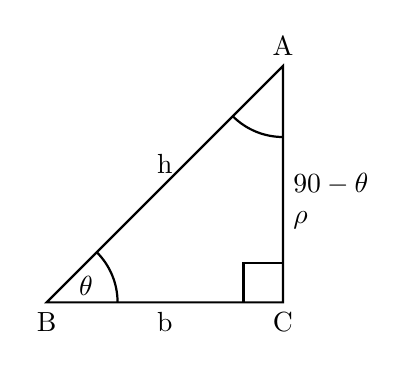
\begin{tikzpicture}[thick]
  % Draw the triangle
  \coordinate (A) at (3,3);
  \coordinate (B) at (0,0);
  \coordinate (C) at (3,0);

  \draw (A) -- node[midway, above]{h}
  (B) -- node[midway, below]{b}
  (C) -- node[midway, right]{$90-\theta$} cycle;

  % additional labels
  \node[above] at (A) {A};
  \node[below] at (B) {B};
  \node[below] at (C) {C};
  \draw (3.0, 0.8) node[above right]{$\rho$};

  % Draw angles
  \pic [draw, angle radius=9mm, "$\theta$"] {angle = C--B--A};
  \pic [draw, angle radius=9mm] {angle = B--A--C};
  \pic [draw, thick] {right angle = A--C--B};
\end{tikzpicture}

\paragraph{Example 3.}
Solve

\begin{enumerate}[label=\arabic*)]
  \item
        \[
        \begin{aligned}
          \sin^{2}(-\alpha) &= \sin(-\alpha) \sin(-\alpha) \\
                            &= (-\sin\alpha)(-\sin\alpha) \\
                            &= \sin^{2}\alpha
        \end{aligned}
        \]
  \item
        \[
        \begin{aligned}
          \cos^{2}(-\alpha) &= \cos(-\alpha) \cos(-\alpha) \\
                            &= (\cos\alpha)(\cos\alpha) \\
                            &= \cos^{2}\alpha
        \end{aligned}
        \]
  \item
        \[
        \begin{aligned}
          \cos\theta \cos(-\theta) - \sin\theta \sin(-\theta) &= \cos\theta \cos\theta - \sin\theta(-\sin\theta) \\
                            &= \cos^{2}\theta + \sin^{2}\theta \\
                            &= 1
        \end{aligned}
        \]
\end{enumerate}

\end{document}
